\documentclass[aspectratio=169]{beamer}
\usepackage[utf8]{inputenc}
\usepackage{lmodern}
\usepackage{tikz}
\usepackage{hyperref}
\usetikzlibrary{positioning,arrows.meta,calc}
\definecolor{tealpop}{HTML}{14B8A6}
\definecolor{goldpop}{HTML}{F4B400}
\definecolor{berrypop}{HTML}{E85D75}
\definecolor{indigopop}{HTML}{5B6CFF}
\definecolor{ink}{HTML}{1F2937}
\definecolor{fog}{HTML}{F7FAFC}
\setbeamertemplate{navigation symbols}{}
\setbeamercolor{normal text}{fg=ink,bg=white}
\setbeamercolor{frametitle}{fg=ink,bg=white}
\setbeamercolor{block title}{fg=white,bg=indigopop}
\setbeamercolor{block body}{fg=ink,bg=fog}
\setbeamertemplate{itemize item}{\color{berrypop}$\blacktriangleright$}
\setbeameroption{hide notes}
\title{Block Coding with Sphero}
\subtitle{Student Mission Deck}
\author{Pine Brook IGNITE}
\date{Spring 2026}
\begin{document}

\begin{frame}[plain]
\begin{tikzpicture}[remember picture,overlay]
\fill[fog] (current page.south west) rectangle (current page.north east);
\fill[tealpop!15] (0.2,0.5) rectangle (13.2,6.9);
\draw[line width=8pt, color=berrypop] (0.5,6.8) -- (12.7,6.8);
\draw[line width=8pt, color=goldpop] (0.5,0.7) -- (12.7,0.7);
\end{tikzpicture}
\vspace{0.55cm}
\begin{center}
{\Huge\bfseries\color{ink} Block Coding with Sphero\par}
\vspace{0.15cm}
{\Large\color{indigopop} Challenge Time: Build, Test, Improve.\par}
\vspace{0.3cm}

\begin{tikzpicture}
\node[rounded corners=18pt, fill=white, draw=indigopop, line width=1.4pt, minimum width=10.6cm, minimum height=1.55cm, text width=9.8cm, align=center]
{\Large\bfseries These learners can handle richer challenges when examples, checkpoints, and debugging moves stay visible.};
\end{tikzpicture}
\vspace{0.35cm}

\begin{tikzpicture}[node distance=0.5cm]
\node[rounded corners=12pt, fill=berrypop!15, draw=berrypop!80, minimum width=3.2cm, minimum height=1.1cm, align=center] (a) {\large\bfseries Notice};
\node[rounded corners=12pt, fill=goldpop!18, draw=goldpop!80!black, minimum width=3.2cm, minimum height=1.1cm, align=center, right=of a] (b) {\large\bfseries Build};
\node[rounded corners=12pt, fill=tealpop!18, draw=tealpop!80!black, minimum width=3.2cm, minimum height=1.1cm, align=center, right=of b] (c) {\large\bfseries Explain};
\end{tikzpicture}
\end{center}
\note{Today we are working on block coding with sphero}
\end{frame}

\begin{frame}[plain]
\frametitle{Mission Goal}
\begin{columns}[T,totalwidth=\textwidth]
\column{0.56\textwidth}
\begin{block}{Today we will}
\Large I can follow the steps.
\end{block}
\begin{itemize}\large
\item I can follow the steps.
\item I can make or improve something.
\item I can show my learning.
\end{itemize}
\column{0.4\textwidth}
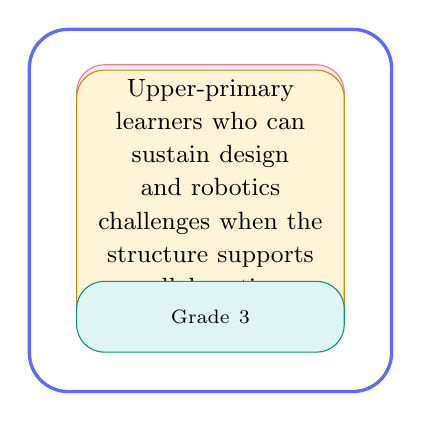
\begin{tikzpicture}[x=1cm,y=1cm]
\draw[rounded corners=14pt, fill=white, draw=indigopop, line width=1.2pt] (0,0) rectangle (4.6,4.6);
\node[draw=berrypop!80, fill=berrypop!14, rounded corners=10pt, minimum width=3.4cm, minimum height=0.9cm] at (2.3,3.7) {\bfseries Grade 3};
\node[draw=goldpop!80!black, fill=goldpop!16, rounded corners=10pt, minimum width=3.4cm, minimum height=1.0cm, text width=3.0cm, align=center] at (2.3,2.35) {\small Upper-primary learners who can sustain design and robotics challenges when the structure supports collaboration and debugging.};
\node[draw=tealpop!80!black, fill=tealpop!14, rounded corners=10pt, minimum width=3.4cm, minimum height=0.9cm, text width=3.0cm, align=center] at (2.3,0.95) {\scriptsize Grade 3};
\end{tikzpicture}
\end{columns}
\note{Today we are working on block coding with sphero}
\end{frame}

\begin{frame}[plain]
\frametitle{Mission Map}
\begin{center}
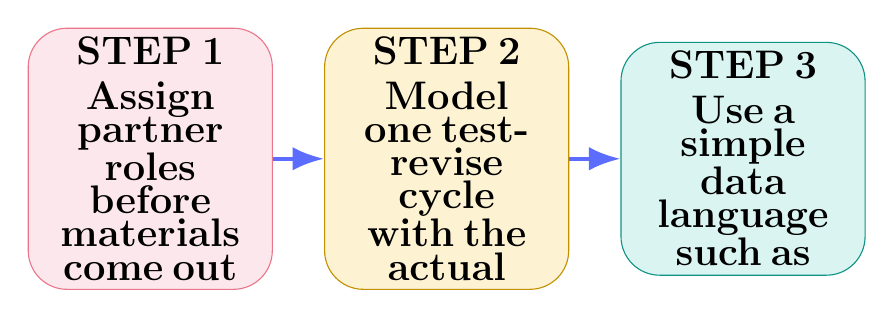
\begin{tikzpicture}[node distance=0.65cm]
\node[rounded corners=14pt, fill=berrypop!14, draw=berrypop!85, minimum width=3.1cm, minimum height=2.0cm, text width=2.4cm, align=center] (s1) {\Large\bfseries STEP 1\\[4pt]Assign partner roles before materials come out};
\node[rounded corners=14pt, fill=goldpop!18, draw=goldpop!80!black, minimum width=3.1cm, minimum height=2.0cm, text width=2.4cm, align=center, right=of s1] (s2) {\Large\bfseries STEP 2\\[4pt]Model one test-revise cycle with the actual};
\node[rounded corners=14pt, fill=tealpop!16, draw=tealpop!80!black, minimum width=3.1cm, minimum height=2.0cm, text width=2.4cm, align=center, right=of s2] (s3) {\Large\bfseries STEP 3\\[4pt]Use a simple data language such as};
\draw[-{Latex[length=4mm,width=3mm]}, line width=1.6pt, color=indigopop] (s1) -- (s2);
\draw[-{Latex[length=4mm,width=3mm]}, line width=1.6pt, color=indigopop] (s2) -- (s3);
\end{tikzpicture}
\end{center}
\vspace{0.28cm}
\begin{block}{Tools and setup}
\begin{itemize}\large
\item Open with a short model that names the lesson focus:
\item Keep one visible success criterion or checklist posted during work
\item End with one observable proof move: explain, submit, save, demonstrate,
\end{itemize}
\end{block}
\note{Use the help routine before you panic}
\end{frame}

\begin{frame}[plain]
\frametitle{Checkpoint and Help Moves}
\begin{columns}[T,totalwidth=\textwidth]
\column{0.52\textwidth}
\begin{block}{If something feels hard}
\begin{enumerate}\large
\item Check the mission map.
\item Re-read the direction.
\item Ask your partner what step you are on.
\item Ask one clear question.
\end{enumerate}
\end{block}
\column{0.43\textwidth}
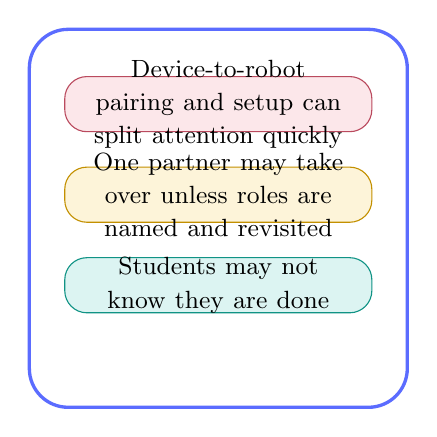
\begin{tikzpicture}[x=1cm,y=1cm]
\draw[rounded corners=14pt, fill=white, draw=indigopop, line width=1.2pt] (0,0) rectangle (4.8,4.8);
\foreach \y/\txt/\col in {3.85/Device-to-robot pairing and setup can split attention quickly/berrypop,2.7/One partner may take over unless roles are named and revisited/goldpop,1.55/Students may not know they are done/tealpop} {
  \draw[rounded corners=8pt, fill=\col!15, draw=\col!80!black] (0.45,\y-0.35) rectangle (4.35,\y+0.35);
  \node[text width=3.3cm, align=center] at (2.4,\y) {\small \txt};
}
\end{tikzpicture}
\end{columns}
\note{Use the help routine before you panic}
\end{frame}

\begin{frame}[plain]
\frametitle{Show Your Learning}
\begin{center}
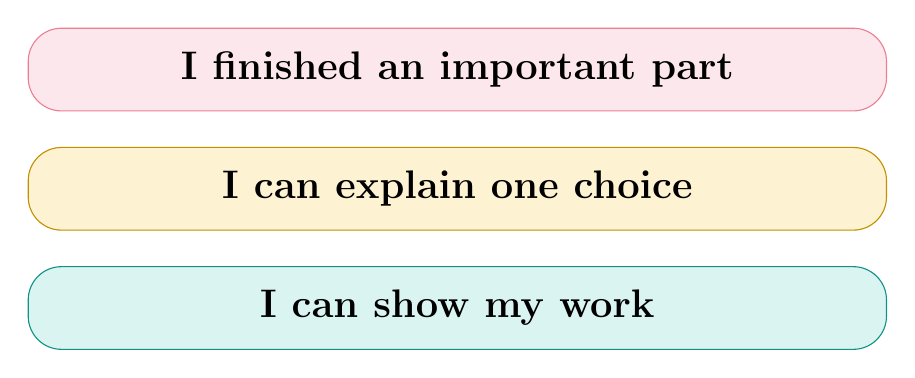
\begin{tikzpicture}[node distance=0.45cm]
\node[rounded corners=12pt, fill=berrypop!14, draw=berrypop!80, minimum width=10.9cm, minimum height=1.05cm, align=center] (a) {\Large\bfseries I finished an important part};
\node[rounded corners=12pt, fill=goldpop!18, draw=goldpop!80!black, minimum width=10.9cm, minimum height=1.05cm, align=center, below=of a] (b) {\Large\bfseries I can explain one choice};
\node[rounded corners=12pt, fill=tealpop!16, draw=tealpop!80!black, minimum width=10.9cm, minimum height=1.05cm, align=center, below=of b] (c) {\Large\bfseries I can show my work};
\end{tikzpicture}
\end{center}
\vspace{0.3cm}
\begin{block}{End-of-lesson move}
\Large Save it, show it, point to it, or explain it in your own words.
\end{block}
\note{Show what you learned at the end}
\end{frame}

\end{document}
